\documentclass[a4paper]{article}
\usepackage[pdftex]{graphicx}
\usepackage{anysize}
\marginsize{3cm}{3cm}{3cm}{3cm}
\linespread{1.2}
\usepackage[utf8]{inputenc}
\usepackage[T1]{fontenc}       
\usepackage[swedish]{babel}      
\usepackage{epstopdf}     % För svensk avstavning och svenska
\usepackage[osf]{mathpazo} % Palatino with smallcaps and oldstyle numbers
\usepackage[scaled]{helvet}
\usepackage{float}
\restylefloat{table}
\usepackage{etoolbox}

\newcommand\getcurrentref[1]{%
 \ifnumequal{\value{#1}}{0}
  {??}
  {\the\value{#1}}%
}  
\newcommand\requirement[2]{
	\numberedrow{Krav}{#1}{#2}
}
\newcommand\scenario[2] {
	\numberedrow{Scenario}{#1}{#2}
}
\newcommand\numberedrow[3]{
	\noindent
	\textbf{#1 \getcurrentref{section}.\getcurrentref{subsection}.#2.} #3
	
}

\usepackage{fancyhdr}
\fancyhf{}
\fancyhead[L]{Ansvarig: SG}

\fancyhead[R]{Datum: \today | Version: 0.21 | Dokumentnummer: PUSS144401}


\title{SRS - Software Requirements Specification: NewPussSystem}                  	
\author{Systemarkitektgruppen \\ Martin Lichota | Marcel Tovar Rascon}
\date{}

\begin{document}

\maketitle
\thispagestyle{fancy}
\tableofcontents
\newpage

\section*{Dokumenthistorik}

\begin{tabular}{ l l l p{8.5cm} }
Ver. & Datum & Ansv. & Beskrivning \\\hline
0.1 & 8 september 2014 & SG & Struktur för dokumentet\\
0.2 & 10 september 2014 & SG & Lägga till krav från UG\\
0.3 & 11 september 2014 & SG & Revidera krav samt ändra struktur\\
0.4 & 12 september 2014 & SG & Lade till nya samt reviderade krav\\
0.5 & 12 september 2014 & SG & Lade till nya samt reviderade krav\\
0.6 & 12 september 2014 & SG & Lade till nya samt reviderade krav\\
0.7 & 12 september 2014 & SG & Lade till nya samt reviderade krav\\
0.8 & 12 september 2014 & SG & Lade till nya samt reviderade krav\\
0.9 & 12 september 2014 & SG & Reviderade krav samt lade till scenarion\\
0.10 & 13 september 2014 & SG & Skapade scenarion för projektledning.\\
0.11 & 13 september 2014 & SG & Skapade scenarion för tidrapportmall och lade till krav.\\
0.12 & 14 september 2014 & SG & Administration och tidrapportering är klart.\\
0.13 & 14 september 2014 & SG & Lade till kontextdiagram samt uppdaterade krav under områdena projektledning, kvalitet och projekt.\\
0.14 & 15 september 2014 & SG & 

Uppdaterat efter granskningsprotokoll från TG, UG, och intern gransking i SG.
Uppdaterat formuleringar, kapitel 3.2 och 4. 
Uppdaterat krav, kapitel 6.1, 6.2, 6.3, 6.4, 6.5.
Lagt till nya krav, kapitel 6.3, 6.4, 6.5.
Uppdaterat scenario, kapitel 6.6. \\
0.15 & 16 september 2014 & SG & Uppdaterade design och lade till formulering, kapitel 4.
Lade till krav, kapitel 6.3.
Uppdaterade krav, kapitel 6.6, 7.2.\\
0.16 & 16 september 2014 & SG & Tog bort reduntant krav, kapitel 6.3.
Lade till krav, kapitel 6.3\\
0.17 & 16 september 2014 & SG & Ändrat krav 6.3.18, 6.3.19, scenario 6.4.4, scenario 6.4.1 och scenario 6.4.3. Lagt till krav 6.4.21, 6.4.22 och scenario 6.4.5.\\
0.18 & 21 september 2014 & SG & Större omstrukturering efter formell granskning.
\\
0.19 & 23 september 2014 & SG & Rättade till en del fel (omstruktureringar).
\\
0.20 & 25 september 2014 & SG & Redigerat krav och lagt till nya efter informell granskning.
\\
0.21 & 2 oktober 2014 & SG & Tagit bort krav och scenario om dynamiska tidsrapportsmallar samt redigerat inloggning av flera terminaler.
\\
\end{tabular}
\newpage
\section{Inledning}       
Dokumentet beskriver kraven för NewPussSystem, ett tidrapportingssystem för projekt som diverse användare kan logga in på.

\section{Referensdokument}
\begin{enumerate}
\item SRS - Software Requirements Specification: BaseBlockSystem (Dokumentnummer PUSS12002, version 1.0)
\end{enumerate}
\section{Bakgrund och mål}   
\subsection{Huvudmål}
Huvudmålet är att tillhandhålla ett system där olika användare, såsom projektledare och övriga projektmedlemmar, skall kunna tidrapportera och loggföra det fortgående arbetet i sitt projekt. 

\subsection{Aktörer och deras mål}
\label{bom-aktorer}
Följande aktörer kommer att använda systemet:
\begin{itemize}
\item [] \textbf{Vanlig användare} En vanlig användare är en person med ett konto i systemet.
\item [] \textbf{Projektmedlem(t1,t2,t3)} En vanlig användare kan tilldelas rollen som projektmedlem. Denne kan tidrapportera och har även tillgång till historik rörande den egna samt gruppens totala tidrapportering. T1, t2, och t3 indikerar tre olika projektmedlemsroller, en användare kan bli tilldelad en av dessa av projektledaren eller administratören.
\item [] \textbf{Projektledare} En användare kan tilldelas rollen som projektledare vilket ger den administrativa rättigheter för ett givet projekt. En projektledare kan tillsätta vanliga användare en projektmedlemsroll samt ändra projektmedlemmars roller. Utöver sina rättigheter som projektledare har den all funktionallitet som en projektmedlem besitter.
\item [] \textbf{Administratör} En administratör är en och endast en användare som har befogenheter att lägga till och ta bort andra användare. Administratören tillsätter även projektledare och skapar projektgrupper. Administratören kan varken vara projektmedlem eller projektledare men har utöver detta samma priviligerade rättigheter som projektledare och projektmedlem.
\end{itemize}
\newpage
\section{Terminologi}
\label{terminologi}
Här följer ord och uttryck som används i rapporten och är till för att öka förståelsen.
\begin{itemize}
\item [] \textbf{Administrationsfunktionaliteter:} De funktionalliteter som faller in under administratören. Exempelvis skapa nya användare eller projekt.
\item [] \textbf{Administrativa rättigheter:} Rättigheter att administrera ett projekt. Rättigheter som projektledare har för sitt projekt samt administratören har för alla projekt.
\item [] \textbf{Aktivitet:} Anger vad man har arbetat med.
\item [] \textbf{Aktivitetsruta:} Cellen där aktivitet (raden) och subaktivitet (kolumnen) möts.
\item [] \textbf{Användarlista:} En lista med alla användarnamn och lösenord som är sparade i databasen.
\item [] \textbf{Användarnamn:} Unik indentifikationsfras för att representera en användare i systemet..
\item [] \textbf{Arbetsbelastning:} Detta är den tiden som en person har lagt ner på en given aktivitet. Om någon har lagt ner 2h på att diska under en viss tidsperiod, så är arbetsbelastningen 2h för den perioden och aktiviteten.
\item [] \textbf{Ej inloggad:} En användare som ännu inte har autentiserat sig mot systemet.
\item [] \textbf{Grundmall:} Är den mallen genererad av systemet som innehåller information om användarnamn, projektgruppsnamn, datum, veckonummer, totaltid och signering (se figur 1). Innehåller också vilka fält som kan anges vid en tidrapportering. Denna går inte att välja bort.
\item [] \textbf{Huvudsida:} Med huvudsida avses den första vyn som användaren blir dirigerad till direkt efter inloggning. 
\item [] \textbf{Information:} Med information avses t.ex. användare, lösenord eller tidrapporter.
\item [] \textbf{Inloggad:} En användare som har loggat in är inloggad.
\item [] \textbf{Logga in:} Då en användare identifierar sig mot systemet med användarnamn och lösenord, om systemet godkänner identifieringen loggar användaren in.
\item [] \textbf{Lösenord:} Hemlig fras endast känd för var unik användare samt systemet så användaren kan påvisa sin identitet.
\item [] \textbf{Meny:} Menyn används för navigering. Den finns på alla sidor för en inloggad användare.
\item [] \textbf{Projektadministrationsfunktionaliter:} De funktionalliteter som faller in under en projektledare. Exempelvis att godkänna tidrapporter eller ta fram statestik.
\item [] \textbf{Projektgrupp:} En grupp bestående av projektmedlemmar och projektledare.
\item [] \textbf{Projektroll:} En roll som en Projektmedlem kan ges. T1, t2 eller t3.
\item [] \textbf{Subaktivitet:} Anger vad för typ av arbete man har arbetat med.
\item [] \textbf{T1, T2, T3:} Se Projektroll.
\item [] \textbf{Terminal:} Dator som används för att använda NewPussSystem.
\item [] \textbf{Tidrapport:} En rapport som innehåller arbetsbelasting för en användare under en fix tidperiod bundet till en specefik projektgrupp.
\item [] \textbf{Tidrapporttabell:} En tabell som fylls i vid tidrapportering. 
\item [] \textbf{Totaltid:} Är den summerade tiden i tidrapportstabellen. 
\item [] \textbf{Vy:} Varje sida ,för en inloggad användare, består av menyn samt en vy. En vy presenterar innehållet i den funktionaliteten man tryckt på i menyn.
\end{itemize}
			\begin{figure}[h!]
				\centering
				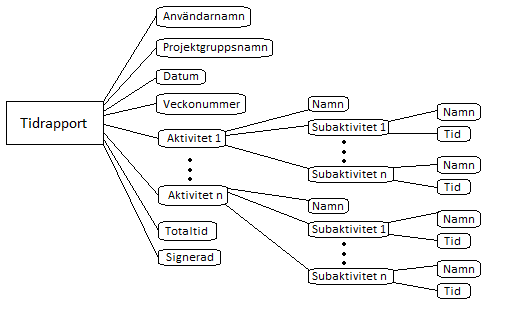
\includegraphics[width=0.75\textwidth]{Tidrapport_Modell}
				\caption{Tidrapportens utseende.}
				\label{image_gen_tidrapport}
			\end{figure}
\section{Kontextdiagram}

\begin{figure}[H]
  \centering
    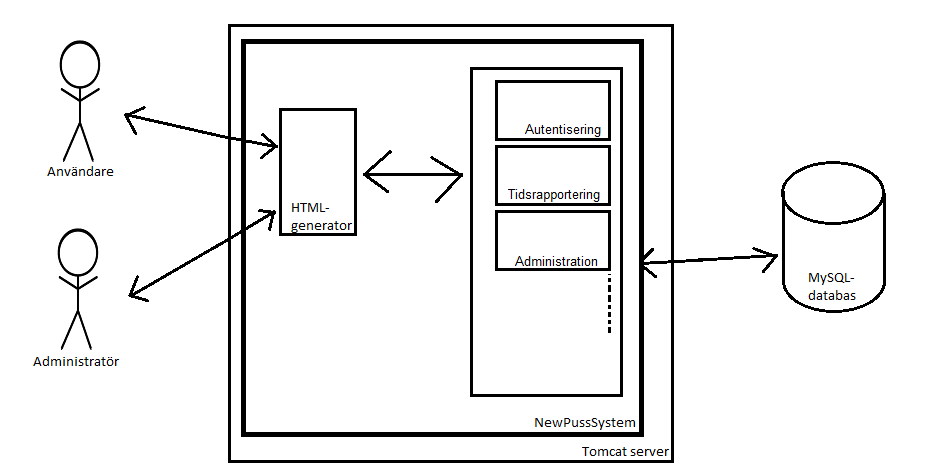
\includegraphics[width=0.75\textwidth]{context}
   \caption{Kontextdiagram för NewPussSystem.}
   \label{image_kontext}
\end{figure}
Kontextdiagram för NewPussSystem illustreras i figur \ref{image_kontext}.

%  _  _______       __      __
% | |/ /  __ \     /\ \    / /
% | ' /| |__) |   /  \ \  / / 
% |  < |  _  /   / /\ \ \/ /  
% | . \| | \ \  / ____ \  /   
% |_|\_\_|  \_\/_/    \_\/    

\section{Funktionella krav}
	\subsection{Generella krav}
		\label{krav-funk-gen}
		\subsubsection*{Användare}
		\requirement{1}{Menyn, oavsett typ av inloggad användare (se avsnitt 3.2), skall vara tillgänglig på samtliga sidor som visas av systemet.}	
		\requirement{2}{Menyn, beroende på typ av inloggad användare (se avsnitt 3.2), skall ge tillgång till de funktionaliteter som denne användaren besitter.}
		\requirement{3}{Menyns innehåll (utifrån krav 6.1.2) skall vara detsamma oavsett vilken sida som visas av systemet.}
		\requirement{4}{Krav 6.4.1 från Grundsystemet (Referensdokument 1) skall stödjas av systemet.}
		\requirement{5}{Det finns sammanlagt fem roller i systemet: administratör, projektledare, t1, t2, t3.}
		\requirement{6}{I varje projektgrupp får det finnas 1-2 projektledare och de tre Projektrollerna, t1, t2 och t3.}
		\subsubsection*{Projektmedlem}		
			\begin{figure}[H]
				\centering
				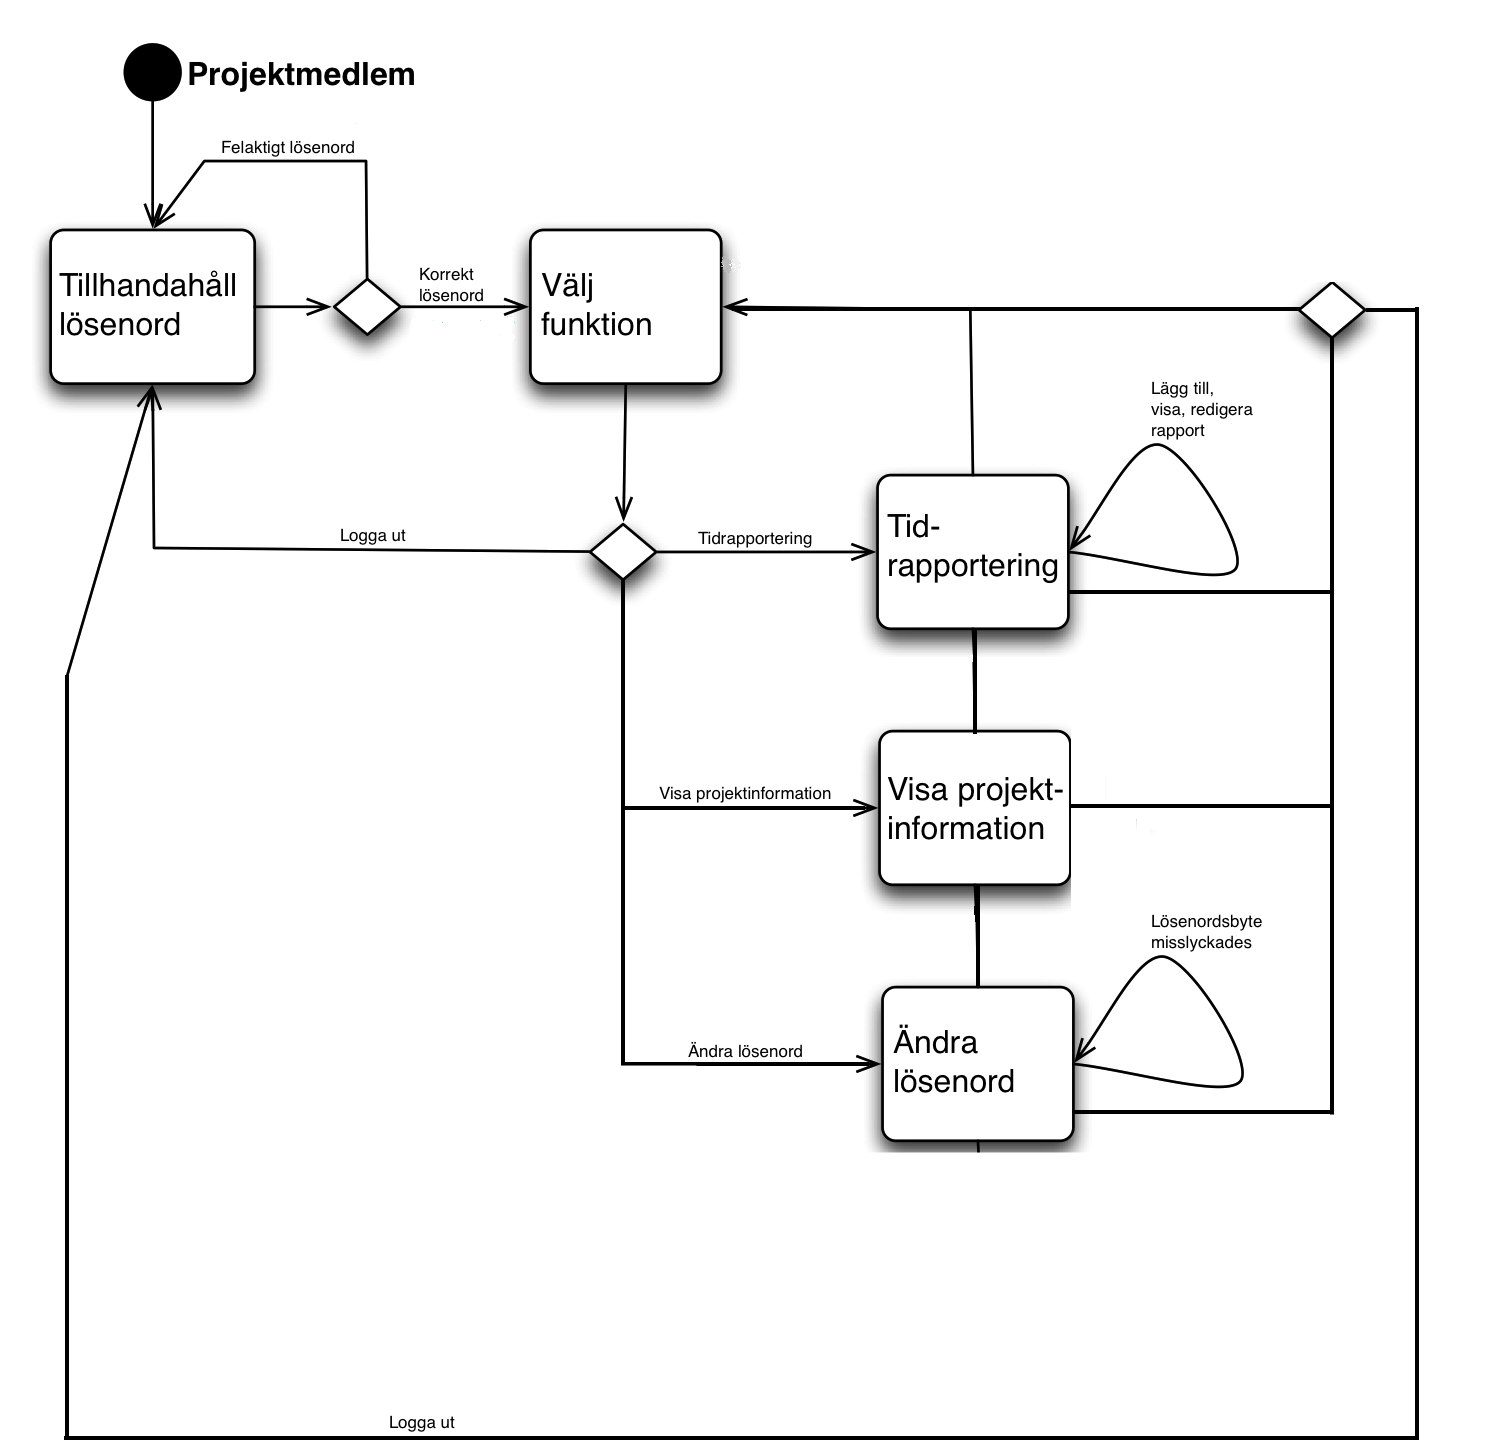
\includegraphics[width=0.75\textwidth]{flow_common_proj_mem}
				\caption{Diagram som visar användarfall för en projektmedlem och projektledare.}
				\label{image_gen_promed}
			\end{figure}
		\requirement{7}{Systemet skall stödja de steg som tas i figur \ref{image_gen_promed}.}
		\subsubsection*{Projektledare}
		\requirement{8}{Varje projekt skall ha en eller två, och endast en eller två, användare som besitter rollen som projektledare.}
		\requirement{9}{Projektledarna har tillgång till projektadministrationsfunktionaliter.}
			\begin{figure}[H]
				\centering
				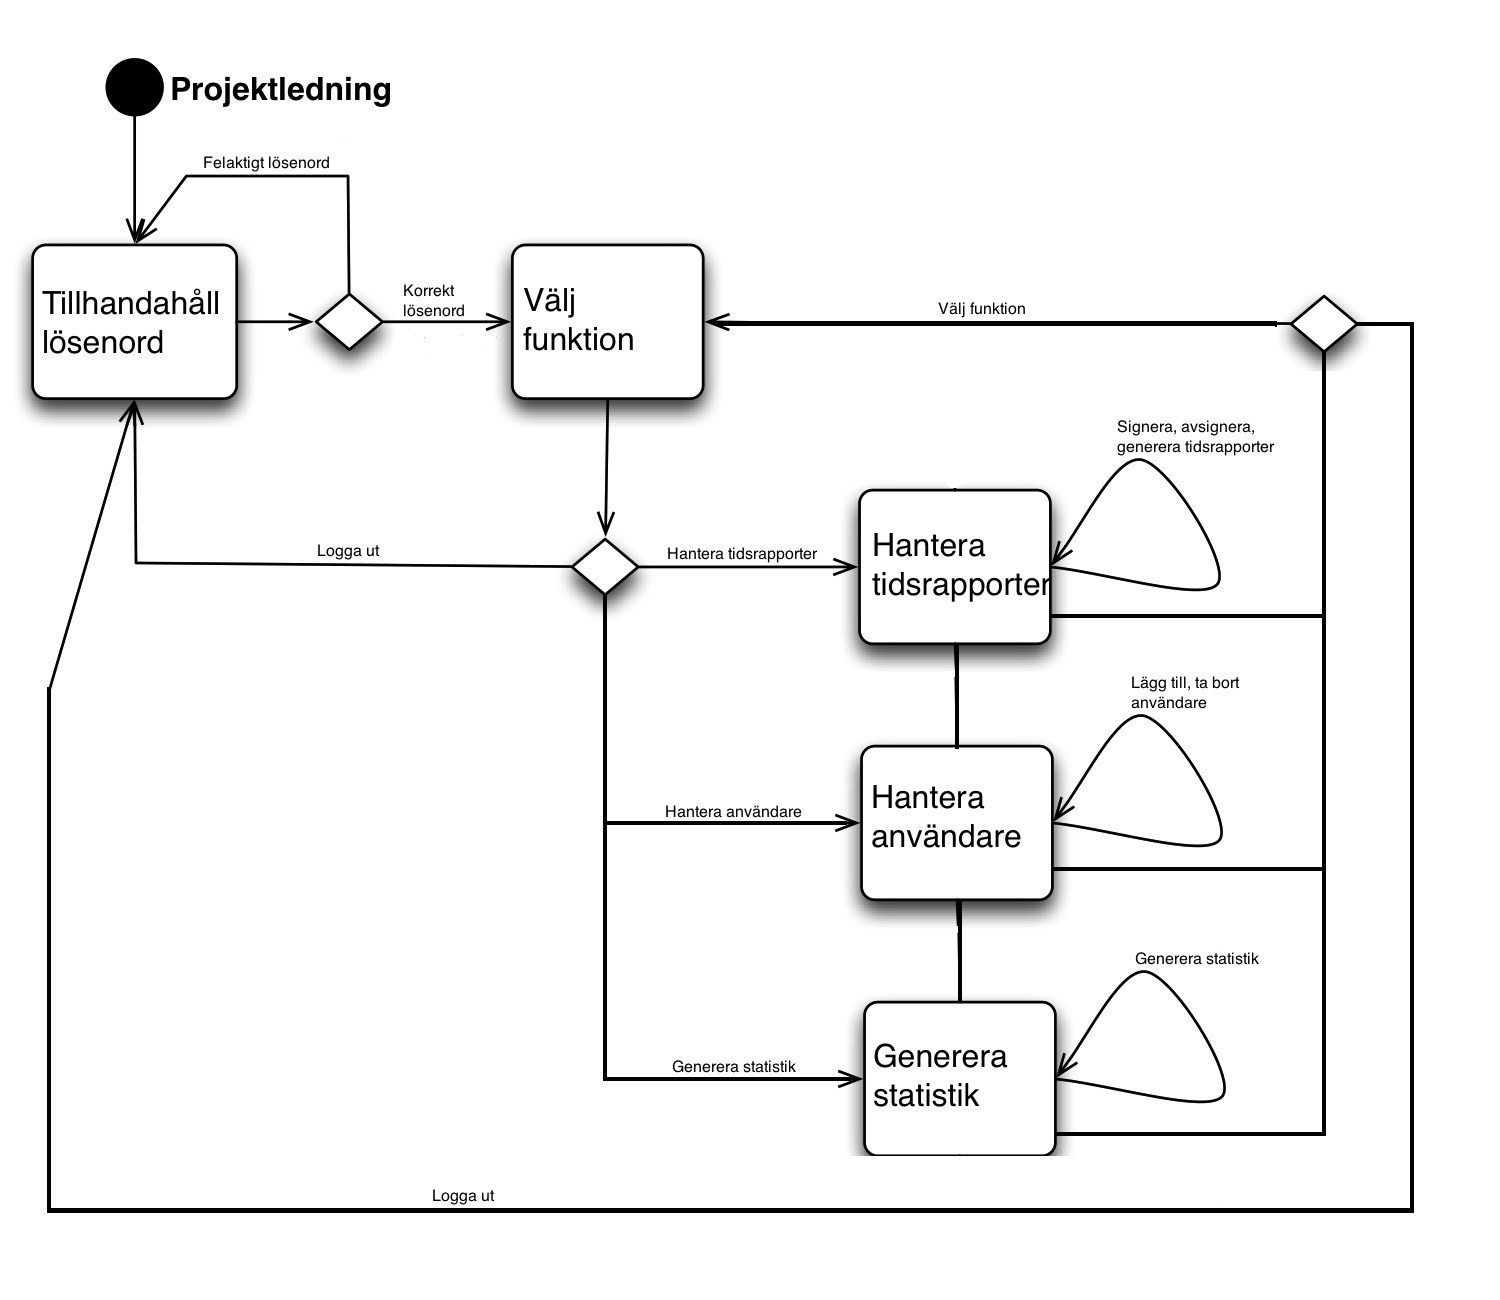
\includegraphics[width=0.75\textwidth]{flow_common_proj_leader}
				\caption{Diagram som visar de utökade användarfallen för en projektledare.}
				\label{image_gen_proboss}
			\end{figure}
		\requirement{10}{Systemet skall stödja de steg som tas i figur \ref{image_gen_proboss}.}
		\subsubsection*{Administratör}
		\requirement{11}{Administratören kan ej vara medlem i en projektgrupp. }
		\requirement{12}{Som inloggad administratör skall det vara möjligt att välja administrationsvyn på huvudsidan.}
			\begin{figure}[H]
				\centering
				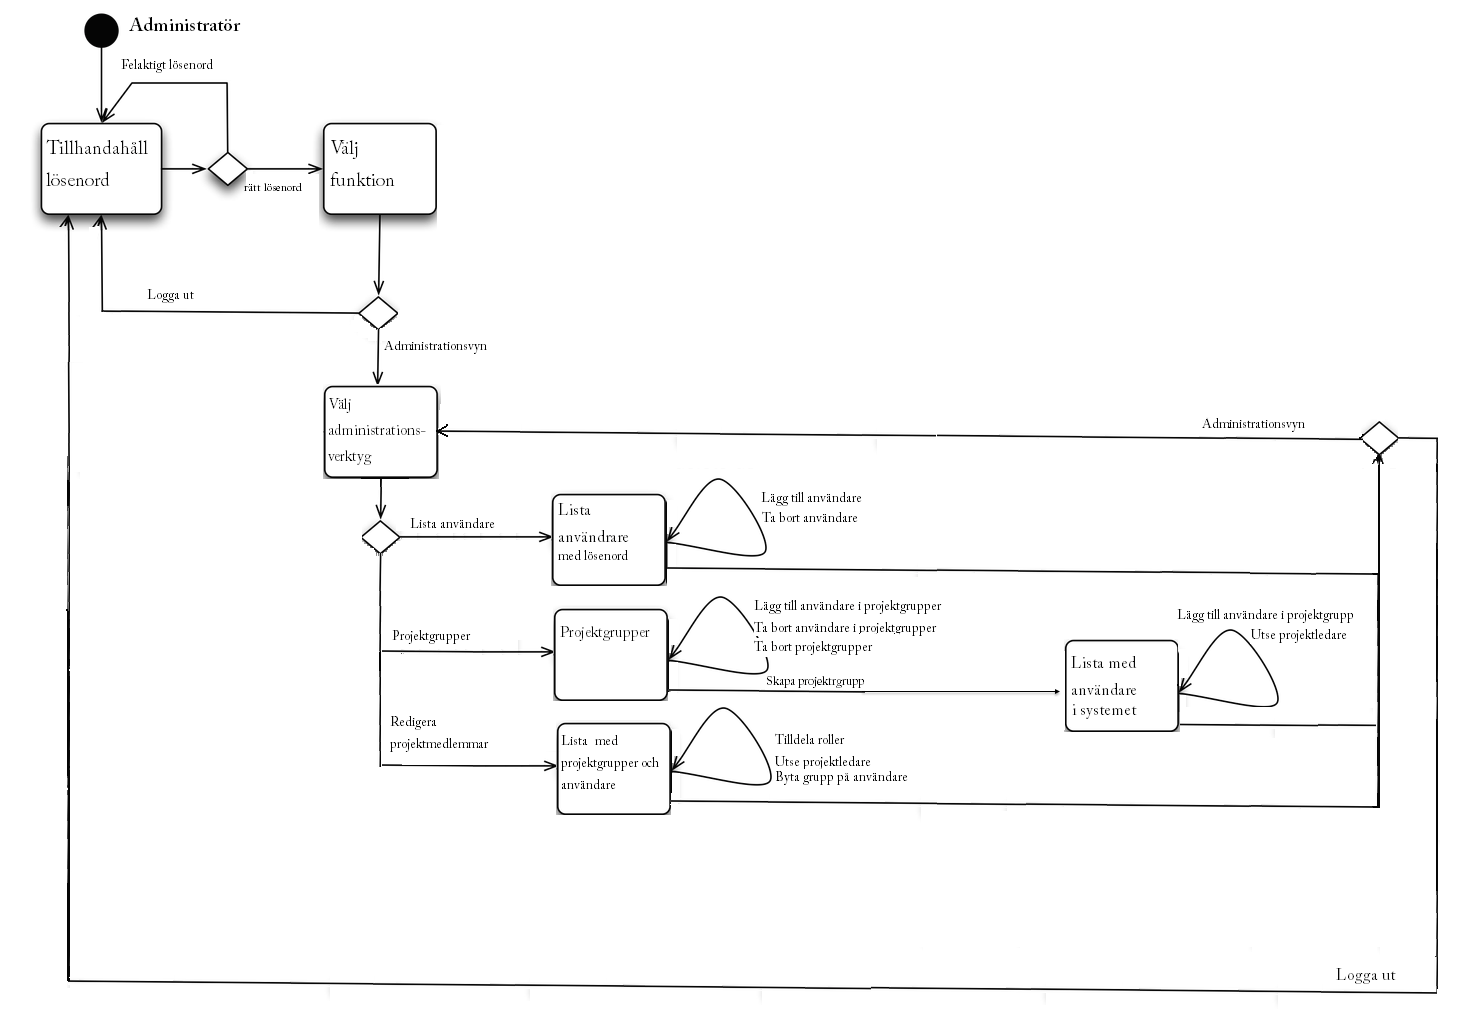
\includegraphics[width=\textwidth]{flow_common_admin}
				\caption{Diagram som visar användarfall för en administratör.}
				\label{image_gen_admin}
			\end{figure}
		\requirement{13}{Systemet skall stödja de steg som tas i figur \ref{image_gen_admin}.}
		\subsubsection*{Data}
		\requirement{14}{Varje borttagning av information skall bekräftas av en dialogruta frågandes om man är säker. Om användaren väljer ``Ja'', tas informationen bort och användaren kommer tillbaka till en uppdaterad sida med informationen. Om ``Nej'' väljs, går användaren tillbaka till nuvarande sida.}
		
		


	\subsection{Autentisering}
		\label{krav-funk-aut}
		\subsubsection*{Övergripande}
			\requirement{1}{Ett användarkonto kan endast vara inloggat på en terminal åt gången.}			
			\requirement{2}{Om en användare försöker logga in med ett användarkonto som redan är inloggat på en annan terminal, kommer den nya inloggningen ej att genomföras. Användaren informeras om detta.}
			\requirement{3}{För varje användare kan loginstatus antingen vara inloggad eller inte inloggad.}

			\requirement{4}{Krav 6.1.2 från Grundsystemet (Referensdokument 1) skall stödjas av systemet.}
			\requirement{5}{Krav 6.2.1 från Grundsystemet (Referensdokument 1) skall stödjas av systemet.}
			\requirement{6}{Krav 6.2.2 från Grundsystemet (Referensdokument 1) skall stödjas av systemet.}
			\requirement{7}{Krav 6.2.3 från Grundsystemet (Referensdokument 1) skall stödjas av systemet.}
			\requirement{8}{Krav 6.2.4 från Grundsystemet (Referensdokument 1) skall stödjas av systemet.}
\subsubsection*{Användare}
			\requirement{9}{Om en inloggad användare är inaktiv i mer än 20 minuter ska denne automatiskt loggas ut från systemet.}
			\requirement{10}{Krav 6.1.3 från Grundsystemet (Referensdokument 1) skall stödjas av systemet.}
			\requirement{11}{Krav 6.1.4 från Grundsystemet (Referensdokument 1) skall stödjas av systemet.}
			\requirement{12}{Krav 6.1.5 från Grundsystemet (Referensdokument 1) skall stödjas av systemet.}
			\requirement{13}{Krav 6.1.8 från Grundsystemet (Referensdokument 1) skall stödjas av systemet.}
			\requirement{14}{Krav 6.1.9 från Grundsystemet (Referensdokument 1) skall stödjas av systemet.}


			
		\subsubsection*{Data}
			\requirement{15}{Krav 6.1.1 från Grundsystemet (Referensdokument 1) skall stödjas av systemet.}
			\requirement{16}{Krav 6.1.7 från Grundsystemet (Referensdokument 1) skall stödjas av systemet.}


		\subsubsection*{Ej inloggad}
			\requirement{17}{Krav 6.1.6 från Grundsystemet (Referensdokument 1) skall stödjas av systemet.}
			\requirement{18}{På inloggningssidan skall användaren ha möjlighet att välja bland alla befintliga projektgrupper i systemet.}
			\requirement{19}{För att kunna utföra autentiseringen mot systemet skall användaren specificera vilken projektgrupp den vill logga in på.}
			\requirement{20}{Användaren skall endast kunna logga in på de projektgrupper denne är medlem i. Detta krav gäller ej för administratören.}



	\subsection{Tidrapportering}
		\label{krav-funk-tid}	
		\subsubsection*{Projektmedlem}
			\requirement{1}{Projektmedlemmar skall kunna skapa, uppdatera och ta bort sina egna osignerade tidrapporter för de projekt de är medlemar i.}
			\requirement{2}{En projektmedlem kan bara se sina egna tidrapporter.}
			\requirement{3}{Projektmedlemmar ska inte kunna ta bort sina signerade tidrapporter.}
			\requirement{4}{Projektmedlemmar ska inte kunna redigera sina signerade tidrapporter.}
			\requirement{5}{Projektmedlemmar ska kunna föra in tidinformation i en aktivitetsruta.}
			\requirement{6}{Projektmedlemmar ska kunna se sammanlagd arbetstid från valda tidrapporter.}

			
%--------------SCENARIO

\begin{table}[H]
\begin{tabular}{ | p{2cm} p{11cm} | }
    \hline
    
    \multicolumn{2}{|p{13cm}|}{ \indent\scenario{1}} \\
    \textbf{Syfte} & Dokumentera arbetstimmar i systemet.\\
    \textbf{Trigger} & Användaren kommer in på tidrapporteringssidan. \\
    \textbf{Förutsättning} & Användaren måste vara medlem i ett projekt.\\
    \hline

	\multicolumn{2}{|p{13cm}|}{\textbf{Subuppgifter}:} \\

	\multicolumn{2}{|p{13cm}|}{1. Användaren väljer tidrapportering.}\\
	\multicolumn{2}{|p{13cm}|}{2. Ett fält där användaren kan fylla i veckonummer för veckan som skall tidrapporteras 	visas. Under fältet framgår det för vilken vecka senaste rapporten var skapad/reviderad.} \\	
	\multicolumn{2}{|p{13cm}|}{3. Användaren fyller i veckonummer och trycker ``OK''.} \\
	\multicolumn{2}{|p{13cm}|}{4. En ny tidrapport genereras och visas med veckonumret från föregående steg samt dagens datum ifyllt.} \\
	\multicolumn{2}{|p{13cm}|}{5. Användaren kan nu fylla i tidinformation. Användaren bekräftar slutligen genom att trycka på ``Skicka'', längst ner på sidan.}\\
	\multicolumn{2}{|p{13cm}|}{6. Rapporten sparas i databasen. En bekräftelse på att så har skett visas för användaren. Användaren kan även notera totaltiden.}\\ \hline
    \multicolumn{2}{|p{13cm}|}{\textbf{Varianter}: }\\
	\multicolumn{2}{|p{13cm}|}{2a. Det finns ingen tidigare skapad rapport. Detta framgår under fältet. }\\
	\multicolumn{2}{|p{13cm}|}{4a. En tidrapport för det ifyllda veckonumret existerar redan. Rapporten hämtas från databasen och visas för användaren. Denne kan nu redigera rapporten (se scenario 6.3.2).}\\
	\multicolumn{2}{|p{13cm}|}{4b. Det ifyllda veckonumret är otillåtet. Användaren informeras om detta och skickas tillbaka till steg 3. }\\
	\multicolumn{2}{|p{13cm}|}{6a. Felaktig inmatning av tidinformation. Användaren skickas tillbaka till steg 5. }\\
    \hline
\end{tabular}
\end{table}

% ----------------------- /END

%--------------SCENARIO

\begin{table}[H]
\begin{tabular}{ | p{2cm} p{11cm} | }
    \hline
    
    \multicolumn{2}{|p{13cm}|}{ \indent\scenario{2}} \\
    \textbf{Syfte} & Ta bort/redigera arbetstimmar i systemet.\\
    \textbf{Trigger} & Användaren kommer in på tidrapporteringssidan. \\
    \textbf{Förutsättning} & Användaren måste vara medlem i ett projekt.\\
    \hline

	\multicolumn{2}{|p{13cm}|}{\textbf{Subuppgifter}:} \\
	\multicolumn{2}{|p{13cm}|}{1. Användaren väljer ''Ta bort/redigera tidrapport''.}\\
	\multicolumn{2}{|p{13cm}|}{2. Användaren får upp en lista med sina egna tidrapporter. Det framgår tydligt vilka som är signerade/osignerade.} \\	
	\multicolumn{2}{|p{13cm}|}{3. Denne väljer en rapport och trycker ``Redigera''.} \\
	\multicolumn{2}{|p{13cm}|}{4. Tidrapporten visas för användaren och kan nu redigeras. När användaren är klar trycker denne ``OK''.} \\
	\multicolumn{2}{|p{13cm}|}{5. Tidrapporten är nu uppdaterad och användaren dirigeras till en bekräftelse sida. }\\
	\hline
    \multicolumn{2}{|p{13cm}|}{\textbf{Varianter}: }\\
	\multicolumn{2}{|p{13cm}|}{3a. Om rapporten är osignerad kan användaren även välja ``Ta bort''. Användaren får upp en bekräftelseruta, specificerad i krav 6.1.14 och dirigeras till steg 5 om denne trycker ``Ja''. Annars tillbaka till steg 2.}\\
	\multicolumn{2}{|p{13cm}|}{4a. Tidrapporten kan endast redigeras om den är osignerad. Signerade tidrapporter visas men användaren har ingen möjlighet att ändra något. }\\
	\multicolumn{2}{|p{13cm}|}{5a. Felaktig inmatning av tidinformation. Användaren skickas tillbaka till steg 4. }\\
    \hline
\end{tabular}
\end{table}

% ----------------------- /END			
			
			
			\requirement{7}{Scenario 6.3.1 skall stödjas av systemet.}
			\requirement{8}{Scenario 6.3.2 skall stödjas av systemet.}
			\begin{figure}[H]
				\centering
				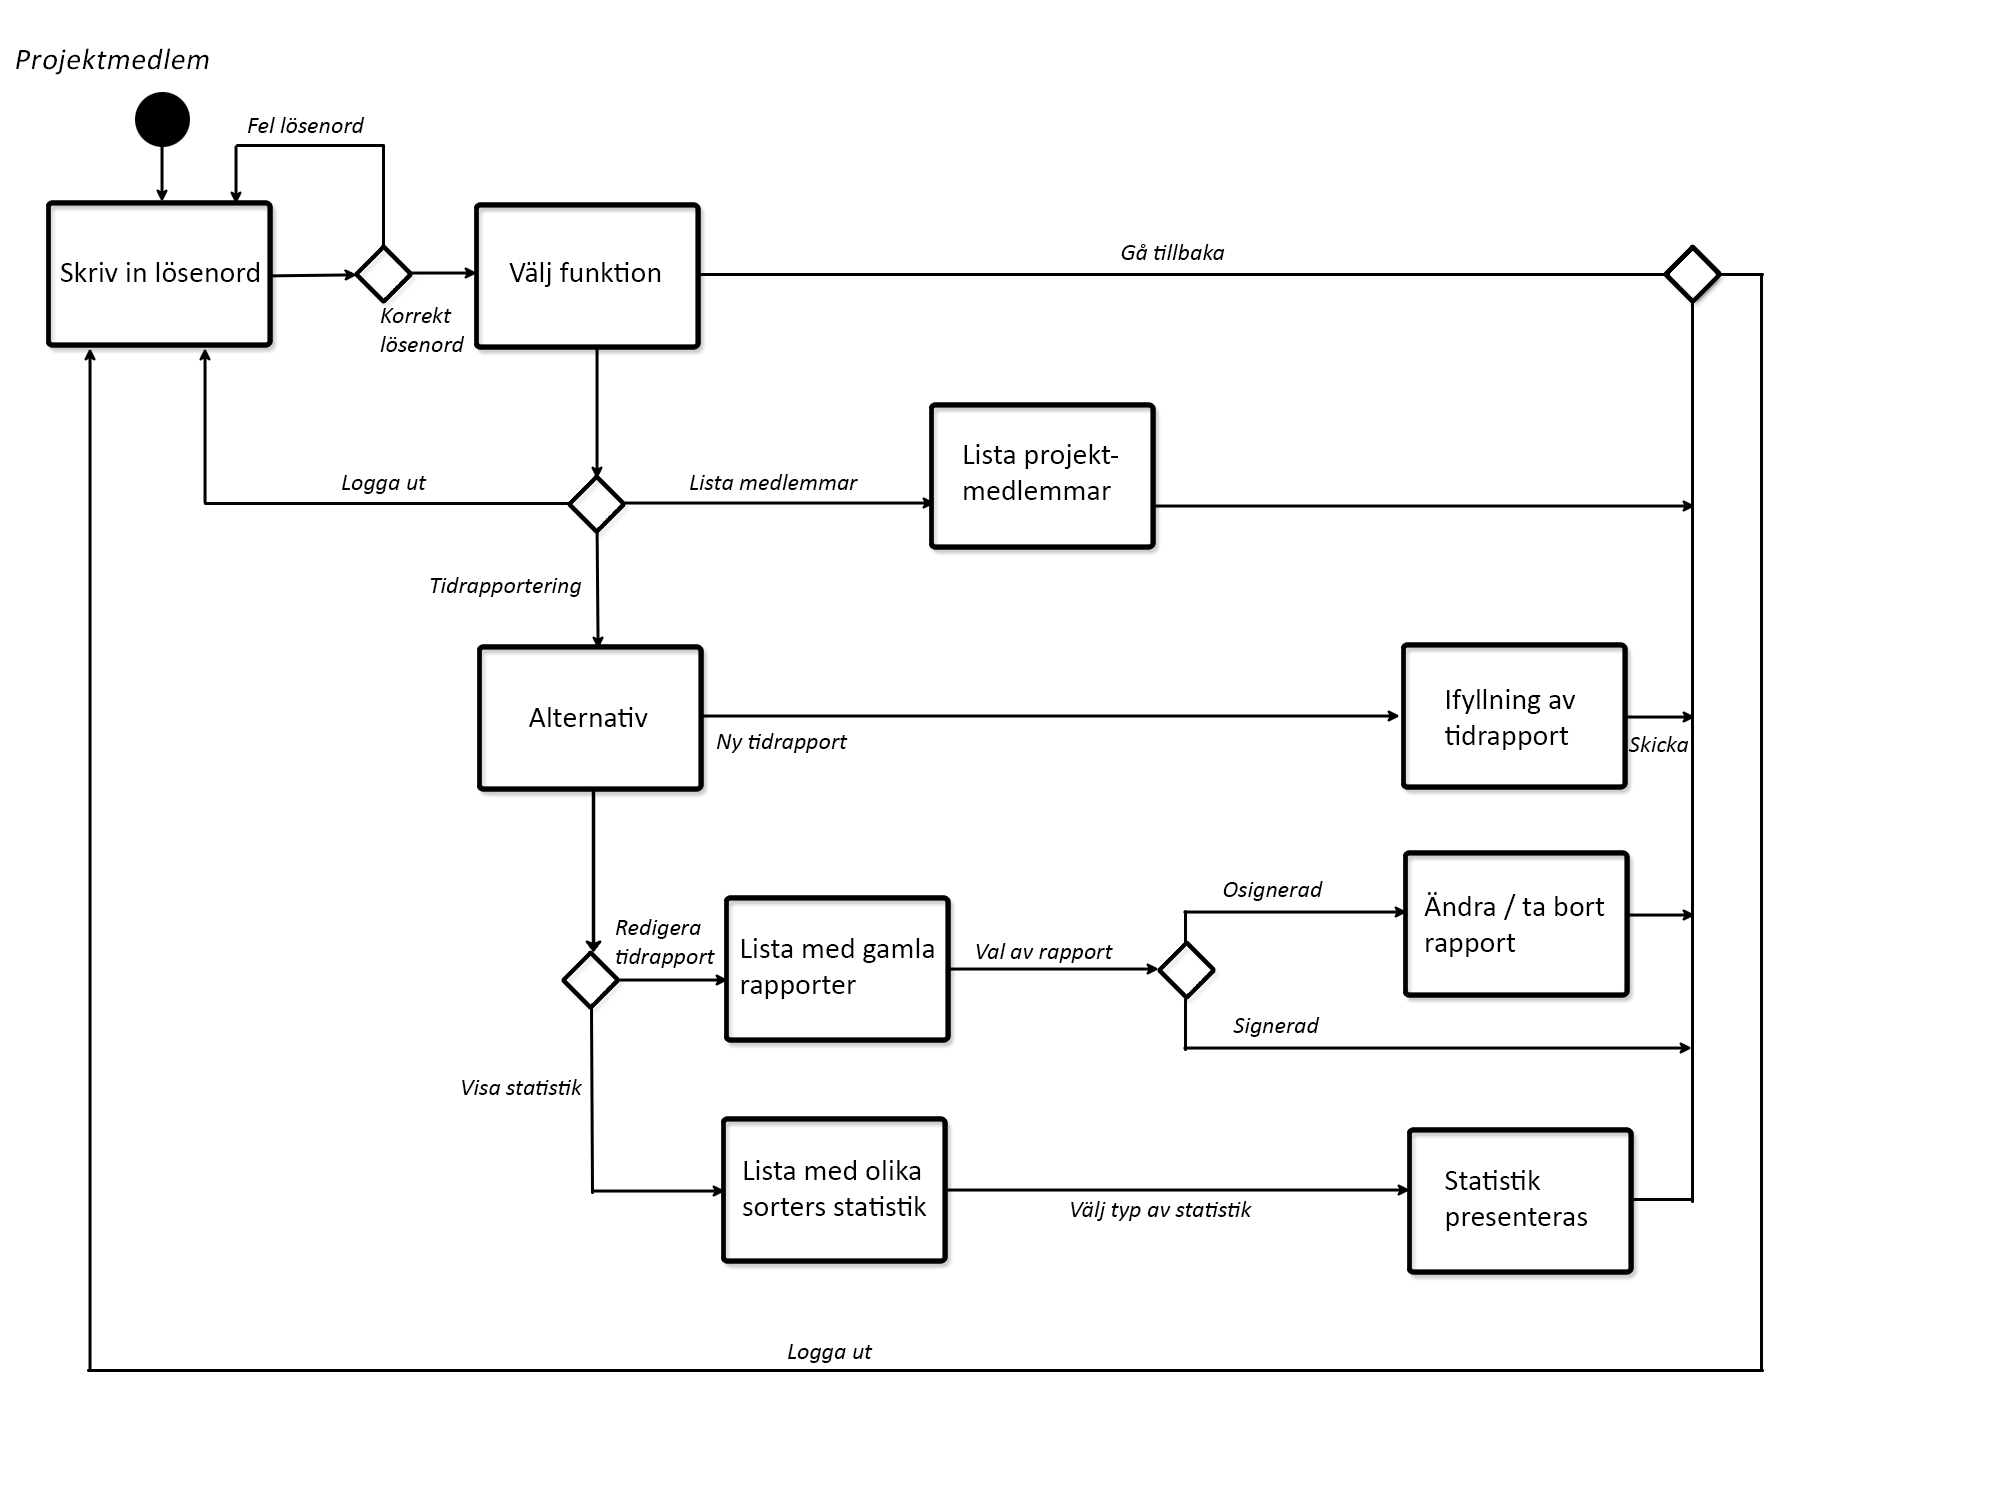
\includegraphics[width=\textwidth]{flow_time_proj_mem}
				\caption{Diagram som visar användarfall för en projektmedlem.}
				\label{image_time_promed}
			\end{figure}
		\requirement{9}{Systemet skall stödja de steg som tas i figur \ref{image_time_promed}.}


		\subsubsection*{Projektledare}
			\requirement{10}{Projektledaren skall ha tillgång till samtliga projektmedlemmars tidrapporter i den projektgrupp den är projektledare för.}
			\requirement{11}{Projektledaren skall kunna godkänna ej tidigare godkända tidrapporter från projektmedlemmar i sin projektgrupp.}
			\requirement{12}{Projektledaren skall kunna ta tillbaka sitt godkännande från en tidigare godkänd gruppmedlems tidrapport, i sin projektgrupp.}
			\requirement{13}{Projektledaren skall kunna generera statistik över sitt projekt genom att summera tidrapporter per användare för samtliga veckor. Med summering menas att summera alla aktivitetsrutor till en ny tidrapport.}
			\requirement{14}{Projektledaren skall kunna generera statistik över sitt projekt genom att summera tidrapporter per roll för samtliga veckor. Med summering menas att summera alla aktivitetsrutor till en ny tidrapport.}
			\requirement{15}{Projektledaren skall kunna generera statistik över sitt projekt genom att summera tidrapporter per aktivitet. Med summering menas att samma aktivitet i alla tidrapporter läggs ihop i en ny tidrapport.}
			\requirement{16}{Projektledaren skall kunna generera statistik över sitt projekt genom att summera tidrapporter per vecka. Med summering menas att summera alla aktivitetsrutor till en ny tidrapport.}
			\requirement{17}{Projektledaren skall kunna generera statistik över sitt projekt genom att summera tidrapporter per användare och aktivitet . Med summering menas att samma aktivitet i alla tidrapporter från samma användare läggs ihop i en ny tidrapport.}
			\requirement{18}{Projektledaren skall kunna generera statistik över sitt projekt genom att summera tidrapporter per användare för utvalda veckor. Med summering menas att summera alla aktivitetsrutor till en ny tidrapport.}
			\requirement{19}{Projektledaren skall kunna generera statistik över sitt projekt genom att summera tidrapporter per roll och aktivitet. Med summering menas att samma aktivitet i alla tidrapporter från samma roll läggs ihop i en ny tidrapport.}
			\requirement{20}{Projektledaren skall kunna generera statistik över sitt projekt genom att summera tidrapporter per roll för utvalda veckor. Med summering menas att summera alla aktivitetsrutor till en ny tidrapport.}
			\requirement{21}{Projektledaren skall kunna generera statistik över sitt projekt genom att summera tidrapporter per aktivitet och vecka Med summering menas att samma aktivitet i alla tidrapporter från samma vecka läggs ihop i en ny tidrapport.}

			\begin{figure}[H]
				\centering
				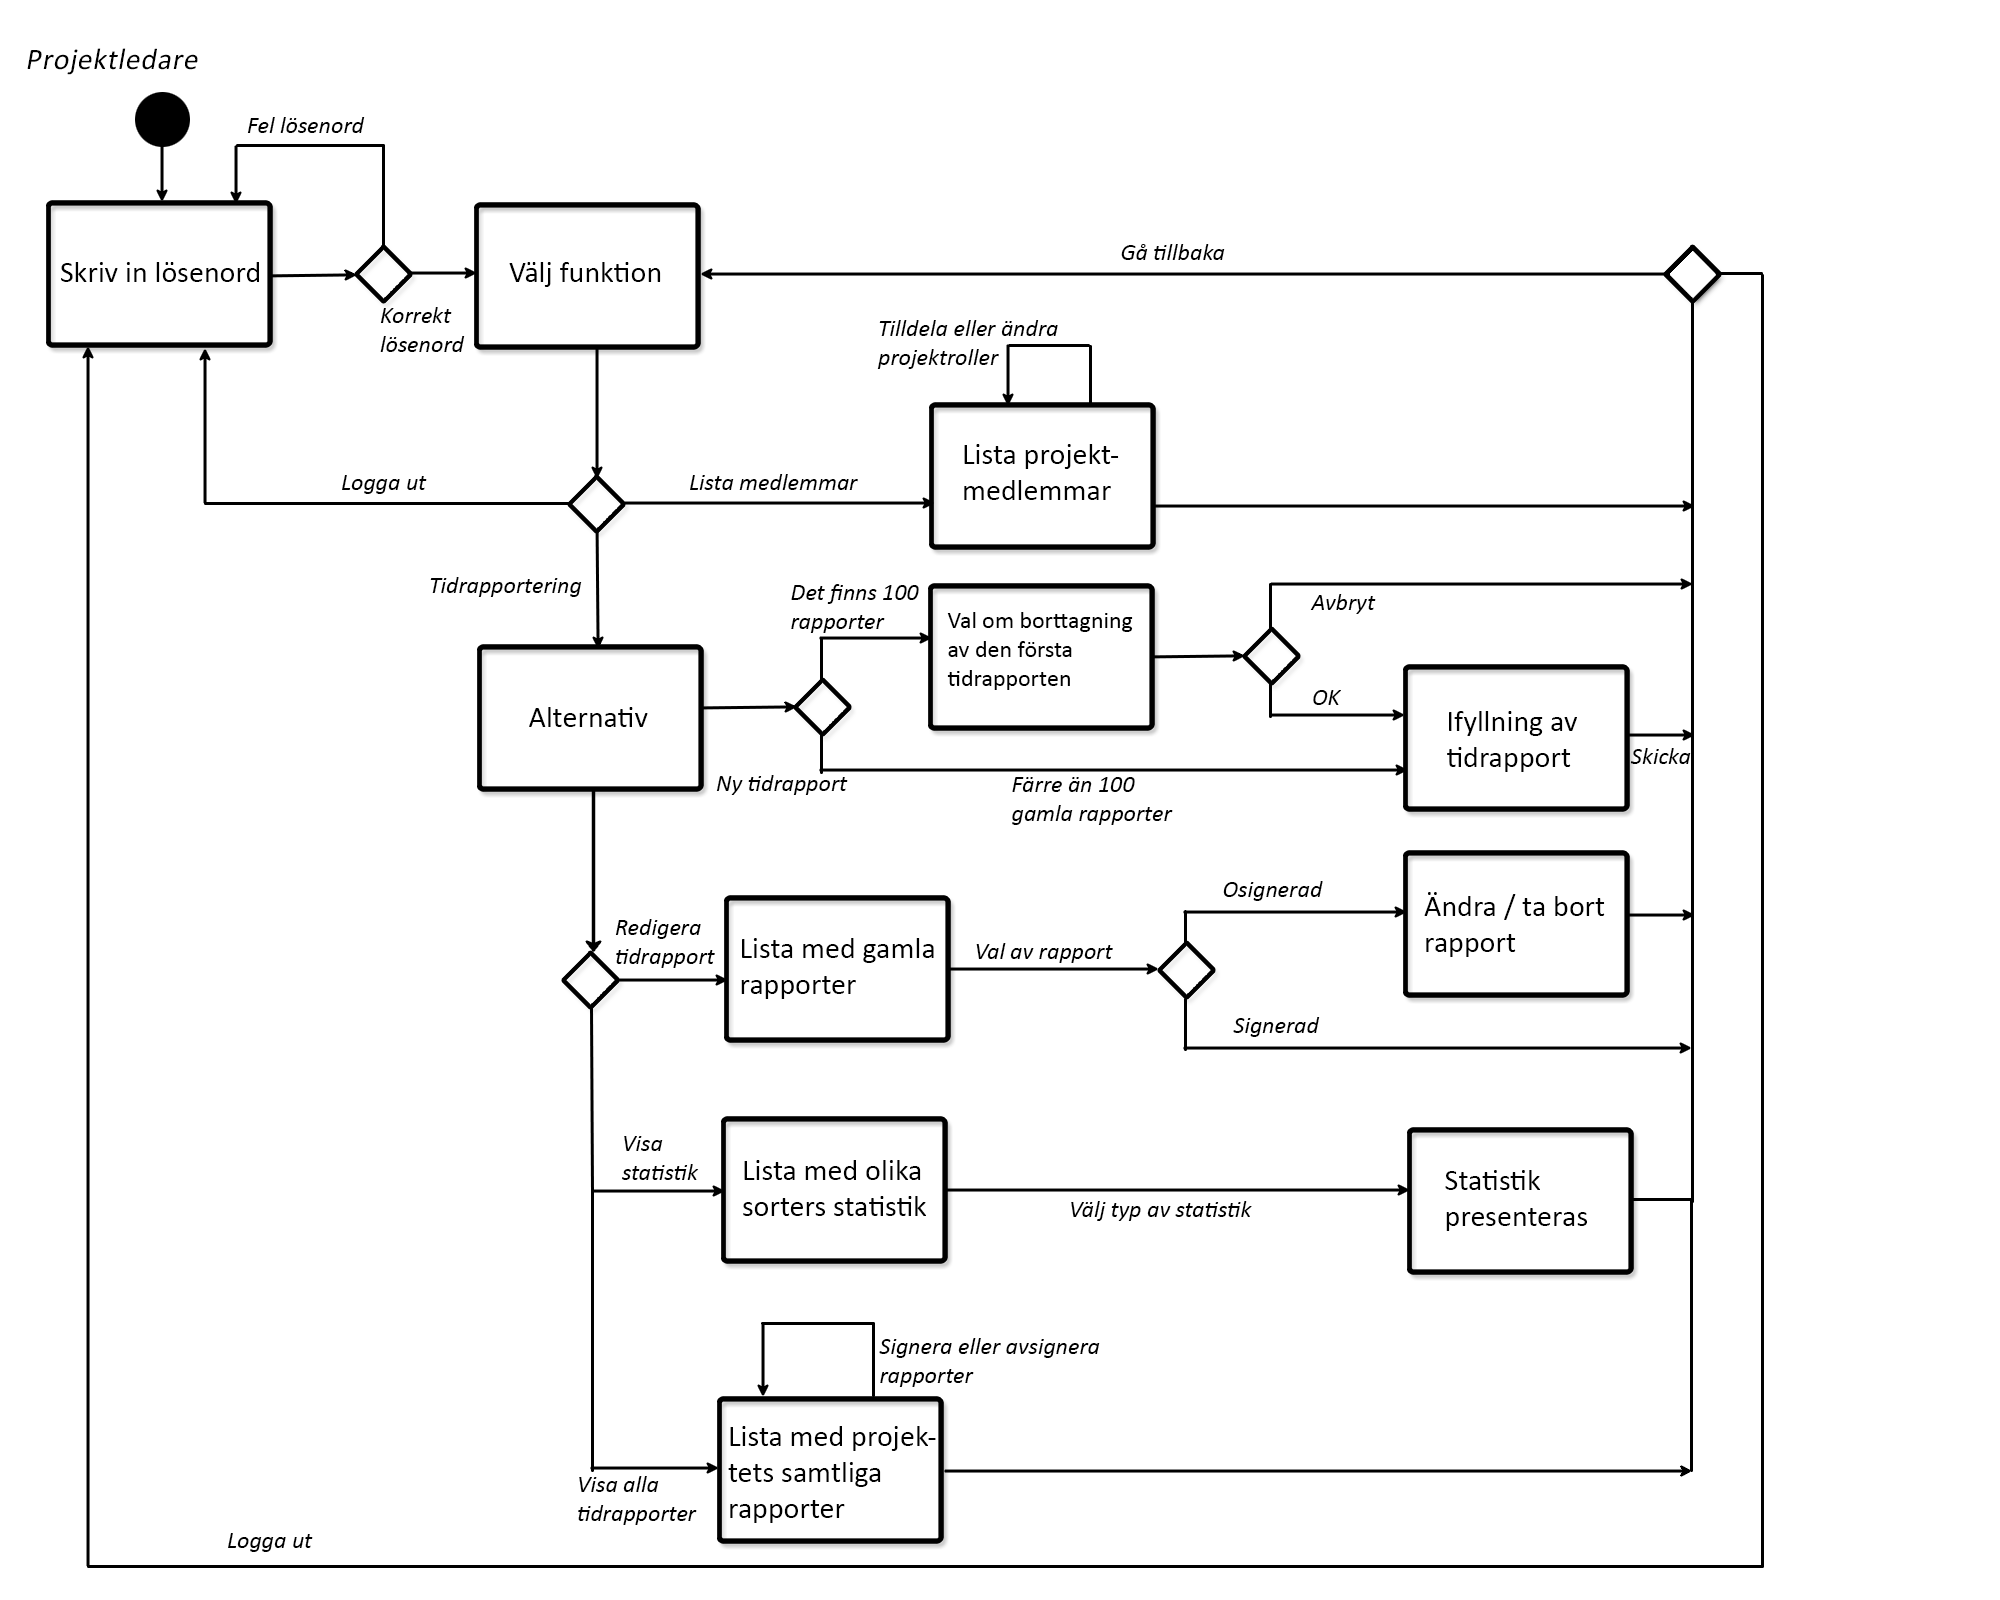
\includegraphics[width=\textwidth]{flow_time_proj_leader}
				\caption{Diagram som visar användarfall för en projektledare.}
				\label{image_time_proboss}
			\end{figure}
		\requirement{22}{Systemet skall stödja de steg som tas i figur \ref{image_time_proboss}.}

		\subsubsection*{Data}
			\requirement{23}{Tidrapportering sker i antal minuter.}
			\requirement{24}{Namnet på aktivitet och subaktivitet ska bestå av 3-5 tecken respektive 1 tecken, ascii (decimal) värden 48-57 och 97-122 är tillåtna.}
			\requirement{25}{Tidinformationen får innehålla 1-5 tecken per aktivitetsruta, ascii (decimal) värden 48-57.}	
			\requirement{26}{Veckonumret får innehålla 1-2 tecken, ascii (decimal) värden 48-57.}
			\requirement{27}{Man skall kunna ange 1-20 stycken aktiviteter i en tidrapportsmall.}
			\requirement{28}{Man skall kunna ange 1-4 stycken subaktiviteter i en tidrapportsmall.}
			\requirement{29}{En tidrapport skall innehålla information om användarnamn.}
			\requirement{30}{En tidrapport skall innehålla information om projektgruppsnamn.}
			\requirement{31}{En tidrapport skall innehålla information om datum. Datum skrivs på formatet ``dag månad år'', där dag representeras av två siffror (ascii (decimal) värden 48-57), månaden som namnet på månaden (ascii (decimal) värden 97-122) , och år med fyra siffor (ascii (decimal) värden 48-57).}
			\requirement{32}{En tidrapport skall innehålla information om veckonummer.}
			\requirement{33}{Det skall tydligt framgå om en tidrapport är signerad eller inte.}
			\requirement{34}{Nygenererade tidrapporter är alltid osignerade.}
			\requirement{35}{Tidrapportens grundmall skall alltid innehålla information om användarnamn, projektgruppsnamn, datum och veckonummer. Det skall även tydligt framgå om den är signerad eller ej.}
			\requirement{36}{Grundmallen för tidrapporterna genereras automatiskt av systemet.}
			\requirement{37}{Aktivitetsnamn måste vara unika.}
			\requirement{38}{Subaktivitetsnamn måste vara unika.}
			\begin{figure}[H]
				\centering
				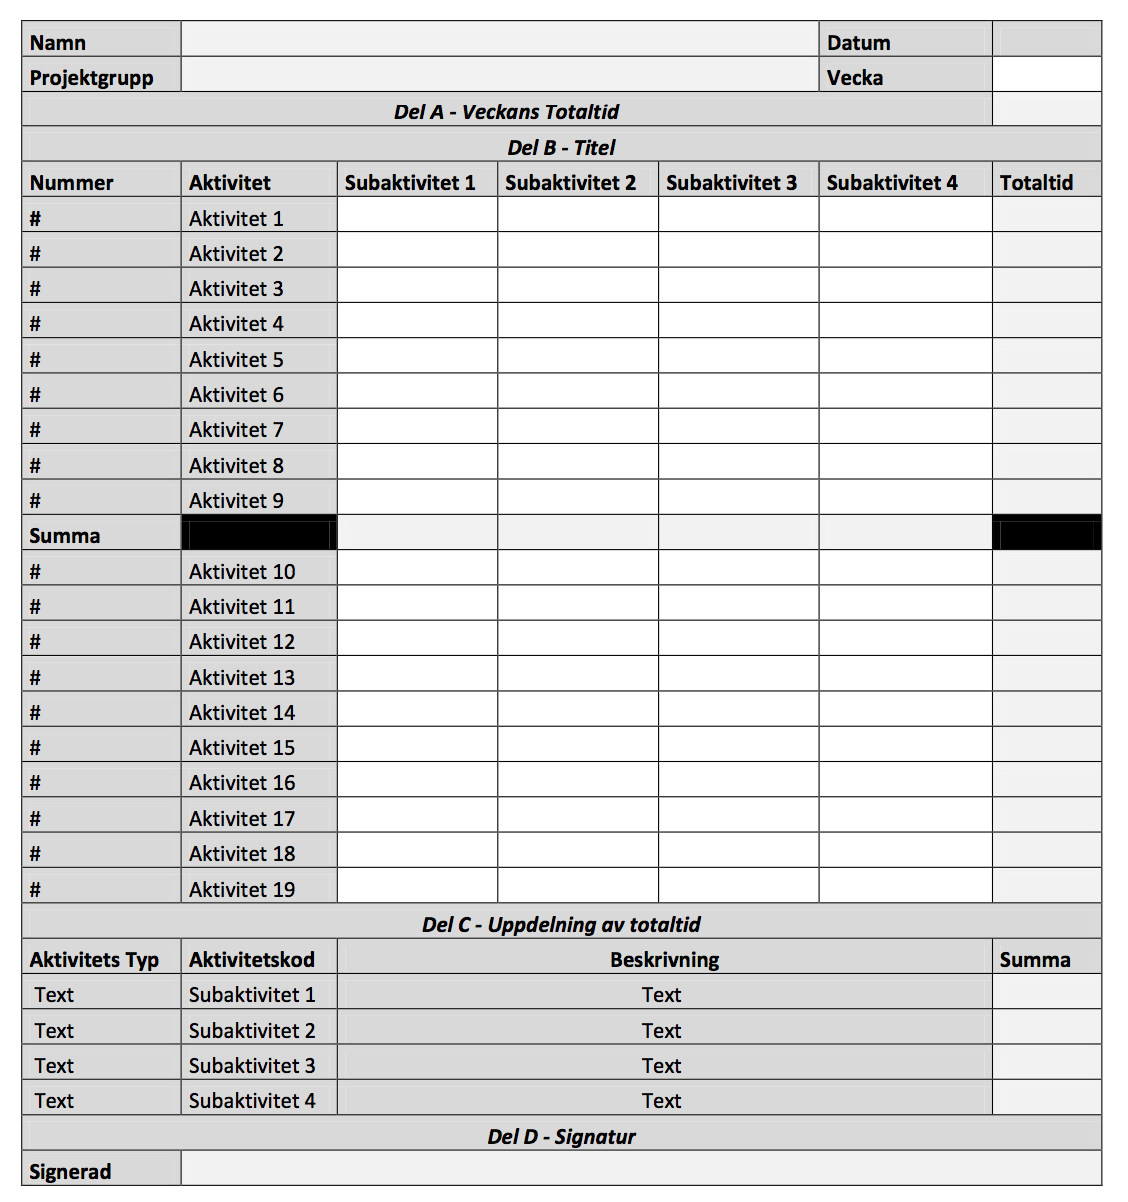
\includegraphics[width=\textwidth]{tidrapportmall}
				\caption{Grundmallen för tidrapporter. Mörkgråa fält är kodade i systemet, ljusgråa fält genereras av systemet, svarta fält ska vara tomma och vita fält fylls i av användaren.}
				\label{image_gen_grundmall}
			\end{figure}
			\requirement{39}{Tidrapporten (grundmallen) ska se ut enligt figur 8.}


	\subsection{Administration}
		\label{krav-funk-admin}
		\subsubsection*{Övergripande}
			\requirement{1}{Krav 6.3.3 från Grundsystemet (Referensdokument 1) skall stödjas av systemet.}		
			\requirement{2}{Krav 6.3.4 från Grundsystemet (Referensdokument 1) skall stödjas av systemet.}
			
		\subsubsection*{Projektledare}
			\requirement{3}{Projektledaren skall kunna tilldela roller till projektmedlemmarna i sin projektgrupp.}
			\requirement{4}{Projektledaren skall kunna lista alla ej godkända tidrapporter.}
			\requirement{5}{Projektledaren skall kunna lista alla godkända tidrapporter.}
			
%--------------SCENARIO

\begin{table}[H]
\begin{tabular}{ | p{2cm} p{11cm} | }
    \hline
    
    \multicolumn{2}{|p{13cm}|}{ \indent\scenario{1}} \\
    \textbf{Syfte} & Generera statistik från systemet.\\
    \textbf{Trigger} & En användare kommer in på statistiksidan för sitt projekt. \\
    \textbf{Förutsättning} & Användaren måste ha rättigheter som en projektledare för det givna projektet.\\
    \hline

	\multicolumn{2}{|p{13cm}|}{\textbf{Subuppgifter}:} \\

	\multicolumn{2}{|p{13cm}|}{1. Användaren väljer statistik.}\\
	\multicolumn{2}{|p{13cm}|}{2. Användaren specificerar vilken/vilka veckor statistiken skall omfatta.} \\	
	\multicolumn{2}{|p{13cm}|}{3. Användaren väljer från en lista vilken typ av rapport den vill generera.} \\	
	\multicolumn{2}{|p{13cm}|}{4. En rapport genereras med statistik efter användarens önskemål} \\
	\multicolumn{2}{|p{13cm}|}{5. Användaren skickas vidare till en sida där den nyligen genererade rapporten visas upp.} \\
		
	\hline

\end{tabular}
\end{table}

% ----------------------- /END
%--------------SCENARIO

\begin{table}[H]
\begin{tabular}{ | p{2cm} p{11cm} | }
    \hline
    
    \multicolumn{2}{|p{13cm}|}{ \indent\scenario{2}} \\
    \textbf{Syfte} & Godkänna en tidrapport.\\
    \textbf{Trigger} & Användaren väljer att lista alla tidrapporter. \\
    \textbf{Förutsättning} & Användaren måste ha rättigheter som en projektledare för det givna projektet.\\
    \hline

	\multicolumn{2}{|p{13cm}|}{\textbf{Subuppgifter}:} \\

	\multicolumn{2}{|p{13cm}|}{1. Användaren väljer en rapport den vill godkänna.}\\
	\multicolumn{2}{|p{13cm}|}{2. Efter att ha kollat igenom rapporten och funnit den ``OK'' väljer den att godkänna.} \\	
	\multicolumn{2}{|p{13cm}|}{3. Användaren trycker på knappen för att godkänna aktuell rapport.} \\
	\multicolumn{2}{|p{13cm}|}{4. En dialogruta beskriver att rapporten blivigt godkänd.} \\
	\multicolumn{2}{|p{13cm}|}{5. Användaren dirigeras tillbaka till sidan över alla tidrapporter.} \\
	
		
	\hline
    \multicolumn{2}{|p{13cm}|}{\textbf{Varianter}: }\\
    \multicolumn{2}{|p{13cm}|}{1a. Rapporten är redan godkänd, se Scenario 6.4.3.}\\    
    \hline
\end{tabular}
\end{table}

% ----------------------- /END
%--------------SCENARIO

\begin{table}[H]
\begin{tabular}{ | p{2cm} p{11cm} | }
    \hline
    
    \multicolumn{2}{|p{13cm}|}{ \indent\scenario{3}} \\
    \textbf{Syfte} & Ta tillbaka godkännande av en tidrapport.\\
    \textbf{Trigger} & Användaren väljer att lista alla tidrapporter. \\
    \textbf{Förutsättning} & Användaren måste ha rättigheter som en projektledare för det givna projektet.\\
    \hline

	\multicolumn{2}{|p{13cm}|}{\textbf{Subuppgifter}:} \\

	\multicolumn{2}{|p{13cm}|}{1. Användaren väljer en rapport den vill godkänna.}\\	
	\multicolumn{2}{|p{13cm}|}{2. Användaren trycker på knappen för att ta tillbaka sitt godkänande av rapporten.} \\
	\multicolumn{2}{|p{13cm}|}{3. En dialogruta beskriver att rapporten ej längre är godkänd.} \\
	\multicolumn{2}{|p{13cm}|}{4. Användaren dirigeras tillbaka till sidan över alla tidrapporter.} \\
		
	\hline
    \multicolumn{2}{|p{13cm}|}{\textbf{Varianter}: }\\
    \multicolumn{2}{|p{13cm}|}{1a. Rapporten är inte godkänd, se Scenario 6.4.2.}\\    
    \hline
\end{tabular}
\end{table}

% ----------------------- /END			
			
			\requirement{6}{Scenario 6.4.1 skall stödjas av systemet.}
			\requirement{7}{Scenario 6.4.2 skall stödjas av systemet.}
			\requirement{8}{Scenario 6.4.3 skall stödjas av systemet.}
			\requirement{9}{Projektledaren skall kunna lista projektets alla tidrapporter och sortera dom efter följande attribut i både stigande och fallande ordning; Användare, vecka, och huruvida rapporten är godkänd eller ej.}

%--------------SCENARIO

\begin{table}[H]
\begin{tabular}{ | p{2cm} p{11cm} | }
    \hline
    
    \multicolumn{2}{|p{13cm}|}{ \indent\scenario{4}} \\
    \textbf{Syfte} & Hitta en rapport genom att sortera dem.\\
    \textbf{Trigger} & Användaren väljer att visa alla tidrapporter för ett projekt. \\
    \textbf{Förutsättning} & Användaren måste ha rättigheter som en projektledare för det givna projektet.\\
    \hline

	\multicolumn{2}{|p{13cm}|}{\textbf{Subuppgifter}:} \\

	\multicolumn{2}{|p{13cm}|}{1. Användaren trycker på valet att sortera alla tidrapporter efter namn, stigande ordning.}\\	
	\multicolumn{2}{|p{13cm}|}{2. Alla tidrapporter visas sorterade efter det givna valet.} \\
	\multicolumn{2}{|p{13cm}|}{3. Användaren trycker på valet att sortera alla tidrapporter efter namn, fallande ordning.} \\
	\multicolumn{2}{|p{13cm}|}{4. Alla tidrapporter visas sorterade efter det givna valet.} \\
	\hline
    \multicolumn{2}{|p{13cm}|}{\textbf{Varianter}: }\\
    \multicolumn{2}{|p{13cm}|}{1a. Användaren väljer istället för namn, att sortera efter vecka.}\\    
    \multicolumn{2}{|p{13cm}|}{1b. Användaren väljer istället för namn, att sortera efter om rapporten är godkänd eller ej.}\\    
    \multicolumn{2}{|p{13cm}|}{3a. Användaren väljer istället för namn, att sortera efter vecka.}\\    
    \multicolumn{2}{|p{13cm}|}{3b. Användaren väljer istället för namn, att sortera efter om rapporten är godkänd eller ej.}\\    
    
    \hline
\end{tabular}
\end{table}

% ----------------------- /END			
			
			\requirement{10}{Scenario 6.4.4 skall stödjas av systemet. }

		\subsubsection*{Administratör}
			\requirement{11}{Administrationsfunktionaliteter avser även projektadministration och därmed har administratörer, utöver sina priviligerade rättigheter, även projektledarnas befogenheter.}
			\requirement{12}{Endast administratören skall kunna skapa projektgrupper i systemet.}
			\requirement{13}{Endast administratören skall kunna lägga till eller ta bort projektledare i en projektgrupp.}
			\requirement{14}{Endast administratören skall kunna ta bort projektgrupper ur systemet.}
			\requirement{15}{När en projektgrupp tas bort elimineras samtliga tidrapporter och tilldelade roller knutna till projektet. Användarna finns kvar i systemet men blir borttagna från den nämnda projektgruppen.}
			\requirement{16}{Scenario 6.4.1 skall stödjas av systemet.}
			\requirement{17}{Scenario 6.4.2 skall stödjas av systemet.}
			\requirement{18}{Scenario 6.4.3 skall stödjas av systemet.}
			\requirement{19}{Scenario 6.4.4 skall stödjas av systemet.}
			\requirement{20}{Scenario 6.4.5 skall stödjas av systemet.}
			\requirement{21}{Krav 6.3.1 från Grundsystemet (Referensdokument 1) skall stödjas av systemet.}
			\requirement{22}{Krav 6.3.5 från Grundsystemet (Referensdokument 1) skall stödjas av systemet.}
			\requirement{23}{Krav 6.3.6 från Grundsystemet (Referensdokument 1) skall stödjas av systemet.}
			\requirement{24}{Krav 6.3.7 från Grundsystemet (Referensdokument 1) har utgått och ersatts av krav 6.1.14}
			\requirement{25}{Krav 6.3.8 från Grundsystemet (Referensdokument 1) skall stödjas av systemet.}
			\requirement{26}{Krav 6.3.9 från Grundsystemet (Referensdokument 1) skall stödjas av systemet.}
			\requirement{27}{Krav 6.3.10 från Grundsystemet (Referensdokument 1) skall stödjas av systemet.}
			\requirement{28}{Krav 6.3.11 från Grundsystemet (Referensdokument 1) skall stödjas av systemet.}
			\requirement{29}{I administrationsvyn skall det vara möjligt att ta bort vilken användare som helst förutom administratören.}
			\requirement{30}{Om en administratör försöker lägga till en ny användare med ett användarnamn som strider mot krav 6.2.5-6 skall ett felmeddelande visas och användaren skall inte läggas till.}
			
%--------------SCENARIO

\begin{table}[H]
\begin{tabular}{ | p{2cm} p{11cm} | }
    \hline
    
    \multicolumn{2}{|p{13cm}|}{ \indent\scenario{5}} \\
    \textbf{Syfte} & Skapa projektgrupp.\\
    \textbf{Trigger} & Användaren vill skapa en projektgrupp. \\
    \textbf{Förutsättning} & Användaren måste vara inloggad som administratör.\\
    \hline

	\multicolumn{2}{|p{13cm}|}{\textbf{Subuppgifter}:} \\

	\multicolumn{2}{|p{13cm}|}{1. Användaren väljer att skapa projektgrupp.}\\
	\multicolumn{2}{|p{13cm}|}{2. Denne får nu fylla i ett projektgruppsnamn och trycker därefter på ``OK''.} \\	
	\multicolumn{2}{|p{13cm}|}{3. Denne möts av en lista över användare i systemet. Första användaren som läggs till tilldelas automatiskt en projektledarroll.} \\	
	\multicolumn{2}{|p{13cm}|}{4. Användaren kan därefter lägga till fler projektgruppsmedlemmar. Det ska även vara möjligt att tilldela ytterligare en projektgruppsmedlem, en projektledarroll. När användaren är klar trycks ``OK''} \\	
	\multicolumn{2}{|p{13cm}|}{5. Projektgruppen skapas och användaren dirigeras till en sida som bekräftar detta. } \\	
	\hline
    \multicolumn{2}{|p{13cm}|}{\textbf{Varianter}: }\\
    \multicolumn{2}{|p{13cm}|}{3a. Projektgruppsnamnet existerar redan, användaren informeras och skickas tillbaka till steg 3.}\\
    \multicolumn{2}{|p{13cm}|}{3b. Projektgruppsnamnet är ogiltligt. Användaren informeras och skickas tillbaka till steg 3.}  \\
    \multicolumn{2}{|p{13cm}|}{3c. Användaren får felmeddelande eftersom inga fler användare existerar. Denne informeras om detta och skickas tillbaka till huvudsidan.}\\
     \multicolumn{2}{|p{13cm}|}{3d. Det går inte att skapa fler projektgrupper då maxgränsen är nådd.
     Användaren informeras om detta.}\\


    \hline
\end{tabular}
\end{table}

% ----------------------- /END



%--------------SCENARIO

\begin{table}[H]
\begin{tabular}{ | p{2cm} p{11cm} | }
    \hline
    
    \multicolumn{2}{|p{13cm}|}{ \indent\scenario{6}} \\
    \textbf{Syfte} & Lägga till/ändra roll på projektmedlem i projektgrupp.\\
    \textbf{Trigger} & Användaren vill lägga till eller ändra projektmedlemmens roll. \\
    \textbf{Förutsättning} & Användaren måste vara inloggad som administratör.\\
    \hline

	\multicolumn{2}{|p{13cm}|}{\textbf{Subuppgifter}:} \\

	\multicolumn{2}{|p{13cm}|}{1. Användaren väljer ''redigera projektmedlemmar''.}\\
	\multicolumn{2}{|p{13cm}|}{2. Användaren får upp en lista med samtliga projektgrupper och projektmedlemmar och en lista med samtliga användare i systemet som inte är projektmedlemmar överhuvudtaget.}\\
	\multicolumn{2}{|p{13cm}|}{3. Användaren har nu möjlighet att flytta över projektmedlemmar och icke projektmedlemmar till olika projektgrupper. Denne kan även ange vilken roll som projekt-medlemmen eller -medlemmarna ska ha.} \\	
	\multicolumn{2}{|p{13cm}|}{4. Användaren bekräftar genom att trycka ``OK''. Denne dirigeras till en sida med den nya informationen samt en bekräftelse.} \\	
	\hline
    \multicolumn{2}{|p{13cm}|}{\textbf{Varianter}: }\\
    \multicolumn{2}{|p{13cm}|}{1a. Det existerar inga projektgrupper/projektmedlemmar. Användaren informeras om detta och skickas tillbaka till huvudsidan.}\\
    \multicolumn{2}{|p{13cm}|}{4a. Användaren får felmeddelande då denne försökt att flytta över en projektledare som är den enda i sin projektgrupp. Denne ombedes att tillsätta en ny projektledare i gruppen innan förflyttning kan äga rum. Användaren dirigeras till steg 3.} \\
    \multicolumn{2}{|p{13cm}|}{4b. Användaren ska informeras om någon av grupperna har max antal användare. Denne ska inte ha möjlighet att lägga till fler projektmedlemmar i den nämnda gruppen. Användaren skickas tillbaka till steg 3.}\\
    \multicolumn{2}{|p{13cm}|}{4c. Om användaren tilldelar en projektmedlem en projektledaroll ska användaren informeras om projektmedlemmens projektgrupp redan har max antal projektledare. Användaren ska då inte ha möjlighet att lägga till fler projektledare i den nämnda projektgruppen. Användaren skickas tillbaka till steg 3.}\\

    \hline
\end{tabular}
\end{table}

% ----------------------- /END



%--------------SCENARIO

\begin{table}[H]
\begin{tabular}{ | p{2cm} p{11cm} | }
    \hline
    
    \multicolumn{2}{|p{13cm}|}{ \indent\scenario{7}} \\
    \textbf{Syfte} & Ta bort projektmedlemmar eller projektgrupp.\\
    \textbf{Trigger} & Användaren väljer ta bort projektgrupp/projektmedlemmar. \\
    \textbf{Förutsättning} & Användaren måste vara inloggad som administratör.\\
    \hline

	\multicolumn{2}{|p{13cm}|}{\textbf{Subuppgifter}:} \\

	\multicolumn{2}{|p{13cm}|}{1. Användaren väljer ta bort projektgrupp/projektmedlemmar.}\\
	\multicolumn{2}{|p{13cm}|}{2. Användaren får upp en lista med samtliga projektgrupper och projektmedlemmar.}\\
	\multicolumn{2}{|p{13cm}|}{3. Användaren markerar projektmedlemmar för borttagning och trycker därefter OK. Bekräftelseruta specificerad i krav 6.1.14 visas och användaren trycker ''Ja''.} \\	
	\multicolumn{2}{|p{13cm}|}{4. Den markerade informationen är nu borttagen och användaren dirigeras till en sida med uppdaterad information.} \\	
	\hline
    \multicolumn{2}{|p{13cm}|}{\textbf{Varianter}: }\\
    \multicolumn{2}{|p{13cm}|}{1a. Det existerar inga projektgrupper/projektmedlemmar. Användaren informeras om detta och skickas tillbaka till huvudsidan.}\\
    \multicolumn{2}{|p{13cm}|}{3a. Användaren trycker ``Nej'' och dirigeras tillbaka till steg 2.} \\
    \multicolumn{2}{|p{13cm}|}{3b. Användaren försöker ta bort en projektmedlem som är ensam projektledare, i en projektgrupp där det åtminstone finns en projektmedlem till. Denne ombedes att tillsätta en ny projektledare och därefter försöka igen. Användaren skickas tillbaka till steg 2.} \\
    \hline
\end{tabular}
\end{table}

% ----------------------- /END
			
			\requirement{31}{Scenario 6.4.6 skall stödjas av systemet.}
			\requirement{32}{Scenario 6.4.7 skall stödjas av systemet.}

		\subsubsection*{Data}
			\requirement{33}{Ett projektgruppsnamn ska bestå av 5-10 tecken, ascii (decimal) värden 48-57 och 97-122 är tillåtna.}
			\requirement{34}{Projektgruppsnamn måste vara unika.}
			\requirement{35}{Det får maximalt existera 5 stycken projektgrupper samtidigt.}
			\requirement{36}{En användare kan vara projektmedlem i mer än en projektgrupp åt gången.}
			\requirement{37}{En projektgrupp skall bestå av 1-20 användare.}
			\requirement{38}{I varje projektgrupp kan det finnas upp till tre Projektroller, t1, t2 och t3.}
			\requirement{39}{I t1, t2 och t3 får det finnas 0-6 användare/projektgrupp, alltså sammanlagt 0-18 användare.}
			\requirement{40}{Krav 6.3.2 från Grundsystemet (Referensdokument 1) skall stödjas av systemet.}


\section{Kvalitetskrav}
	\subsection{Underhåll}
		\requirement{1}{Systemet skall vara väl dokumenterad så det underlättar vidareutvekling av systemet i framtiden.}
		\requirement{2}{Krav 7.1.1 från Grundsystemet (Referensdokument 1) skall stödjas av systemet.}
		\requirement{3}{Förståelse av Java, i nivå med vad som lärs ut i kursen EDA016, samt grundläggande kunskap av SQL skall räcka för att underhålla samt vidareutveckla systemet.}



	\subsection{Prestanda}
		\label{krav-kval-pres}
		\requirement{1}{Systemet skall klara av att få 20 stycken inloggningar under en tidperiod av 1 sekund, utan att bryta mot några andra kvalitetskrav.}
		\requirement{2}{Krav 7.2.1 från Grundsystemet (Referensdokument 1) skall stödjas av systemet.}
		\requirement{3}{Maximalt 50 användare kan vara inloggade på systemet samtidigt.}

	\subsection{Användarvänlighet}
		\requirement{1}{Minst 7/10, på måfå utvalda Civilingenjörsstudenter, skall finna det lätt att använda systemet.}

\section{Projektkrav}
	\subsection{Utvecklingsmiljö}
	\requirement{1}{Krav 8.1.1 från Grundsystemet (Referensdokument 1) skall stödjas av systemet.}
	\requirement{2}{Krav 8.1.2 från Grundsystemet (Referensdokument 1) skall stödjas av systemet.}
	\requirement{3}{Krav 8.1.3 från Grundsystemet (Referensdokument 1) skall stödjas av systemet.}
	\requirement{4}{Systemet samt projekt- och produktdokumentation skall skrivas på svenska. Java- koden skall följa standarden som finns på http://www.geosoft.no/development/javastyle.html, alla variabelnamn skall vara skrivna på engelska.}




\end{document}